\section{Fabric inversion}

The primary observable is the azimuthal velocity pattern
$v(\varphi)$, read through the E1 time of flight
(Figure~\ref{fig:sweepobs}), and the primary inversion
(\cmd{sim/model/fit\_fabric.py}, \cmd{fit\_sweep.py}) recovers fabric
parameters from it in two stages: a coarse global search over fabric
strength and direction followed by local refinement, which avoids the
local minima that a direct descent on the periodic $2\varphi$ pattern
invites. The fit reports the recovered eigenvalue and fast-axis
azimuth with residuals, and the sweep-level tooling fits entire
simulated campaigns unattended.

\begin{figure}[htb]
  \centering
  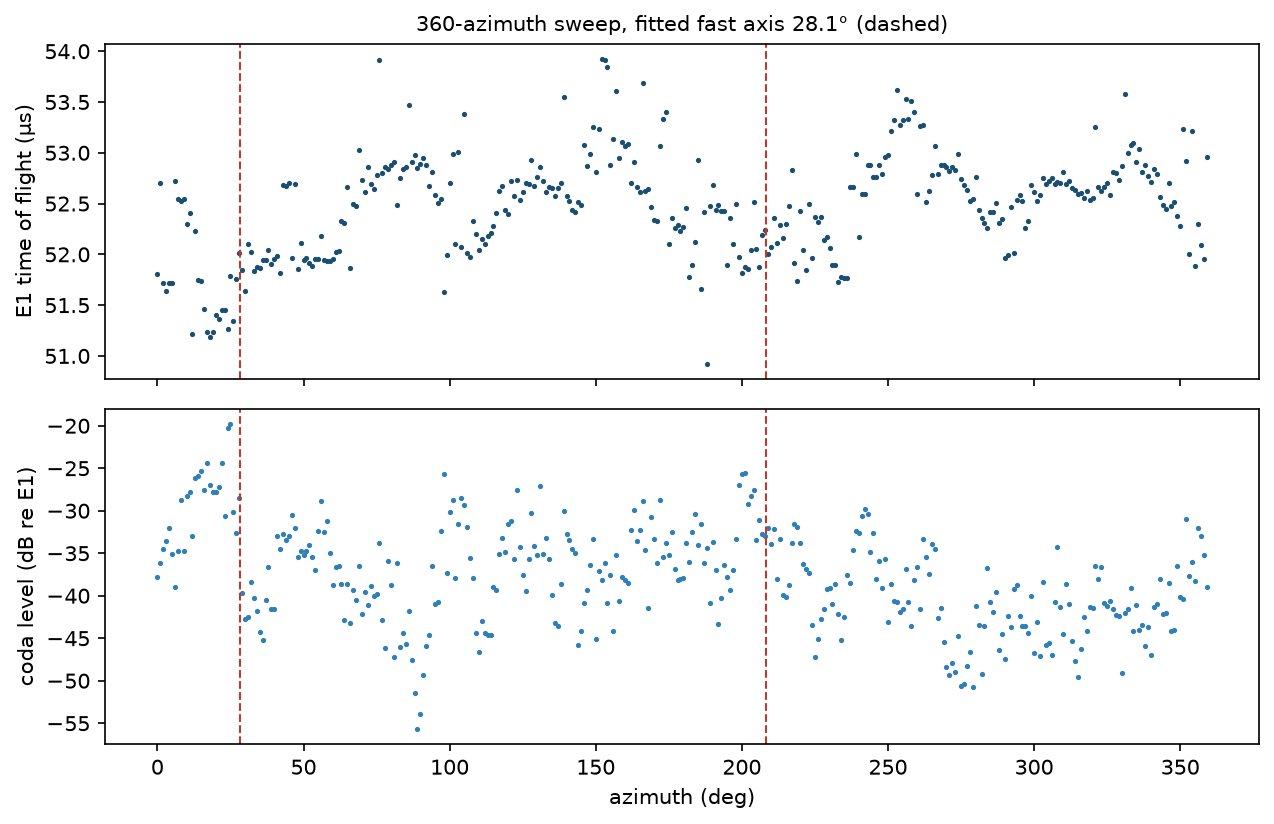
\includegraphics[width=0.95\textwidth]{figures/sweep-observables.png}
  \caption{A complete 360-azimuth full-wave sweep: E1 time of flight
    (top) and coda level (bottom) against azimuth. The
    second-harmonic time-of-flight pattern and the coda elevation
    around the fabric axis are both visible by eye; dashed lines mark
    the fitted fast axis.}
  \label{fig:sweepobs}
\end{figure}

Beyond the single bulk fit, a gridded inversion divides the disk into
regions and inverts per-area fabric, with a daemon that processes
sweeps as they complete. Its purpose is honesty about spatial
resolution: a diametral measurement integrates along chords, so
per-area recovery is only meaningfully constrained where chords
cross, and the gridded results quantify that rather than assert it.
